\documentclass{article}

\usepackage[margin = 1in]{geometry}
\addtolength{\topmargin}{-0.5in}

\usepackage{setspace}
\onehalfspacing

\usepackage{amsmath}
\usepackage{graphicx}
\usepackage{float}

\title{Exchange rate forecasting with the Taylor rule}
\author{Lawrence Leung}
\date{2/10/2021}

\begin{document}

\maketitle

From the uncovered interest rate parity condition, the difference of the logarithm of two countries's interest rates must also be the expected one-period ahead change in the logarithm of the exchange rate. 
\begin{equation}
log(1+i)-log(1+\tilde{i}) = log(\hat{s}_{t+1}) - log(s_t) \approx \%\Delta \hat{s}_{t+1}.
\end{equation}
By using the Taylor Rule as an indicator of what a country's interest rate will be, we can generate forecasts of the 1 period ahead change in exchange rates. The Taylor Rule is
\begin{equation}
i_t^* = \pi_t + \phi(\pi_t-\pi^*) + \gamma(y_t-\bar{y}_t) + r^*,
\end{equation}
where $i_t^*$ is the target short-term nominal interest rate, $\pi_t$ is the current inflation rate, $\pi^*$ is the target level of inflation, $y_t$ is the logarithm of real GDP, $\bar{y}_t$ is the logarithm of potential GDP, and $r^*$ is the equilibrium real interest rate. Since we do not expect interest rates to adjust according to the Taylor Rule immediately, we include each country's lagged interest rate $i_{t-1}$ as a covariate to "smooth out" the model. Assuming that the two countries have the same inflation target and neutral interest rate (symmetry), the model specification we obtain is
\begin{equation}
i_t-i_t^*=w+w_{u\pi}\pi_t-w_{f\pi}\tilde{\pi}_t+w_{uy}y_t-w_{fy}\tilde{y}_t+w_{ui}i_{t-1}-w_{fi}\tilde{i}_{t-1}+\eta_t,
\end{equation}
where $\sim$ indicates foreign variables. 


We use this specification to make one-month ahead forecasts of the CAD:USD and GBP:USD exchange rates. Rolling forecasts are initialized using 120 periods of monthly data starting January 1975 for Canada and March 1973 for the U.K.. At each step, a model is estimated using $OLS$ and the one-period ahead forecast is made. The first data point is then dropped, one data point is added at the end of the sample, and the process is repeated until forecasts for June 2006 are made.


We evaluate the performance of our forecasts with two statistical tests: the Diebold-Mariano-West test and the Clark-West test. The $DMW$ test statistic is
\begin{equation}
DMW = \frac{\hat{\sigma}^2_{rw}-\hat{\sigma}^2_{l}}{\sqrt{\frac{1}{P}\hat{V}}} \sim N(0,1),
\end{equation}
where $\hat{\sigma}^2_{rw}$ is the prediction mean squared error $MSPE$ for a random walk model, $\hat{\sigma}^2_{l}$ is the $MSPE$ for the linear model we are testing, $P$ is the number of predictions, and $\hat{V}=\frac{1}{P}\sum^T_{t=T-P+1} ((s_{t+1}-s^{rw}_{t+1})^2-(s_{t+1}-s^{l}_{t+1})^2 - (\hat{\sigma}^2_{rw}-\hat{\sigma}^2_{l}))^2$, where $s_{t+1}$ and $s^{l}_{t+1}$ are the forecasted exchange rates from the random walk and linear model, respectively. The CW test statistic can be written as a function of the DMW test statistic, that is
\begin{equation}
CW = DMW + \frac{1}{\sqrt{\frac{1}{P}\hat{V}}}\frac{1}{P}\sum^T_{t=T-P+1}(X'_{t+1}\hat{\beta}_t)^2 \sim N(0, 1),
\end{equation}
where $X'_{t+1}\hat{\beta}_t$ is the forecasted change in the logarithm of exchange rate. Results from these two tests are shown in Table 1.

\begin{table}[H] \centering 
  \caption{Symmetric Taylor rule model with smoothing, hetereogenous coefficients, linear trend, constant} 
\begin{tabular}{@{\extracolsep{5pt}} ccccccc} 
\\[-1.8ex]\hline 
\hline \\[-1.8ex] 
 & $\sigma^2_{rw}$ & $\sigma^2_{l}$ & $DMW$ & $p$ & $CW$ & $p$ \\ 
\hline \\[-1.8ex] 
Canada & $1.592 \times 10^{-4}$ & $1.614 \times 10^{-4}$ & $$-$0.248$ & $0.598$ & $2.439^{***}$ & $0.008^{***}$ \\ 
U.K. & $6.245 \times 10^{-4}$ & $6.893 \times 10^{-4}$ & $$-$1.735$ & $0.959$ & $1.898^{**}$ & $0.029^{**}$ \\ 
\hline \\[-1.8ex] 
\textit{Note:} & \multicolumn{2}{r}{$^{*}$p$<$0.1; $^{**}$p$<$0.05; $^{***}$p$<$0.01} \\ 
\end{tabular} 
\end{table}

The $DMW$ test evaluates the null hypothesis that the prediction error from the linear model is no better than that of a random walk. Then the null and alternative hypotheses can be written as follows:
\[\begin{split}
H_0:& \hat{\sigma}^2_{rw} = \hat{\sigma}^2_{l} \\
H_1:& \hat{\sigma}^2_{rw} > \hat{\sigma}^2_{l} \\
\end{split}\]
Using the $DMW$ test, we fail to reject the null that the $MSPE$ from the Taylor rule model is better than the $MSPE$ from a random walk model.


However, one criticism of the $DMW$ test is that it under-rejects the null that the coefficients in the linear model are equal to 0. If the coefficients in the linear model have nonzero coefficients, it would imply that it has some predictive power. Under the $CW$ test, the null and alternative hypotheses are
\[\begin{split}
H_0:& \beta = 0 \\
H_1:& \beta \neq 0 \\
\end{split}\]
Using the $CW$ test, we reject the null that the Taylor rule model has no predictive for both CAD:USD and GBP:USD exchange rates. For the Canadian exchange rate, we reject the null at the $p=0.01$ level and for the U.K. exchange rate, we reject the null at the $p=0.05$ level. Therefore we conclude that in this setting, there is strong evidence in the predictability of interest rates using a model incorporating Taylor rule fundamentals.

\begin{figure}
\centering
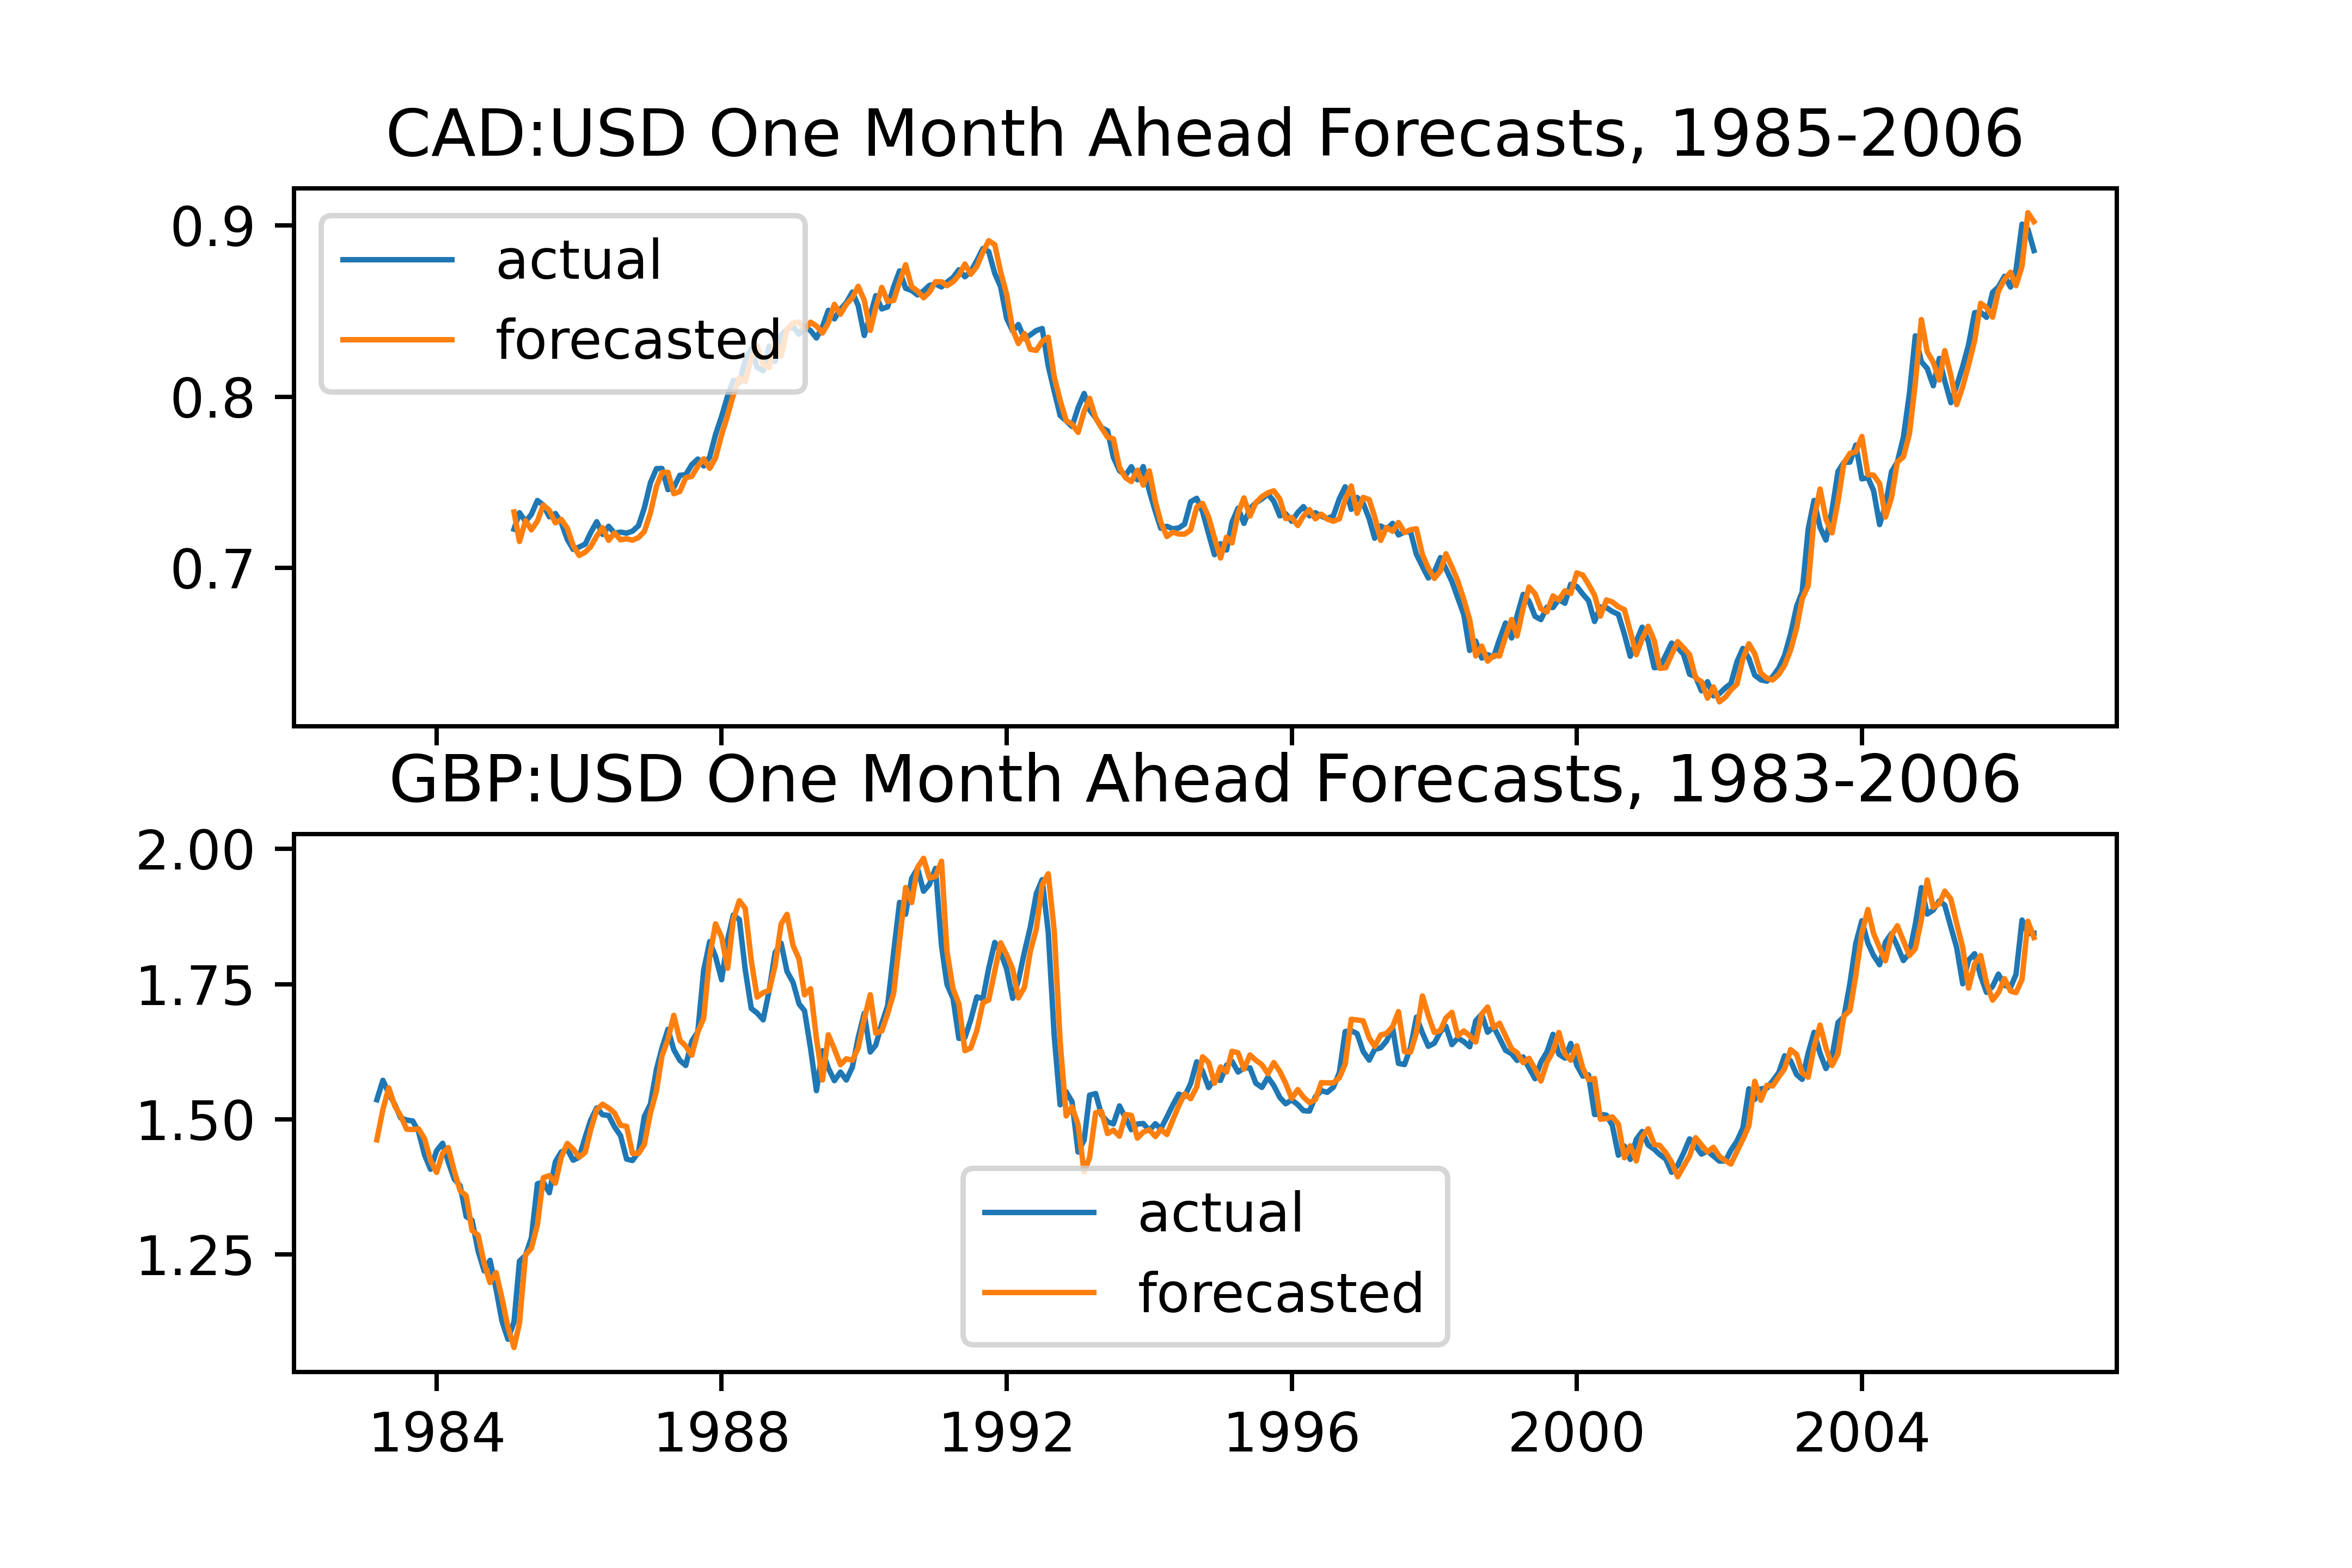
\includegraphics{forecasts.png}
\end{figure}

\end{document}